\documentclass[crop,tikz,border=10px,convert=pdf2svg,multi=false]{standalone}
\usepackage{amsfonts}
\usepackage[defaultsans]{opensans}
\usetikzlibrary{shapes,arrows,positioning}
\begin{document}
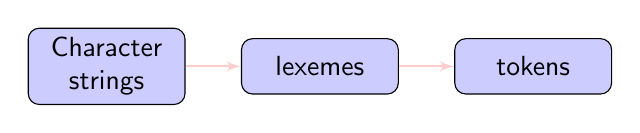
\begin{tikzpicture}[font=\sffamily,node distance=2em,remember picture,
  block/.style = {rectangle, draw, fill=blue!20, text centered, text
    width=5em, rounded corners, minimum height=2em},
  line/.style = {draw, -latex', red!20, thick}]

  \node [block] (n0) {Character strings};
  \node [block, right=of n0] (n1) {lexemes};
  \node [block, right=of n1] (n2) {tokens};

  \draw [line] (n0) -- (n1);
  \draw [line] (n1) -- (n2);

\end{tikzpicture}
\end{document}
